\documentclass{article}
\usepackage[utf8]{inputenc}
\usepackage[margin = 0.8in]{geometry}
\usepackage{graphicx}
\usepackage{amsmath, amssymb}
\usepackage{subcaption}
\usepackage{multirow}
\usepackage{mathtools}
\usepackage{float}


\title{RBE550 - Valet Path Planning Assignment}
\author{Keith Chester}
\date{Due date: March 21 2022}

\begin{document}
\maketitle

\section*{Introduction}
In this assignment, we are tasked with path planning in challenging continuous spaces with unique vehicle-specific kinematic constraints. To accomplish this, we utilize state lattices to explore a continuous space while adhering to the kinematics of each vehicle. Specifically, we explore a skid drive robot, an Ackermann drive robot, and an Ackermann drive robot with hitch-attached trailer.

\section*{Vehicles and Kinematics}

First, we introduce each vehicle type and discuss the kinematics of their movement.

\subsection*{Skid Drive}
This robot is called skid drive as the robot simply skids the front caster wheel around while two drive wheels control its movement. The skid drive robot can turn within its own radius, and can perform curved trajectories by differing the angular velocity of the wheels.

\begin{figure}[H]
    \centering
    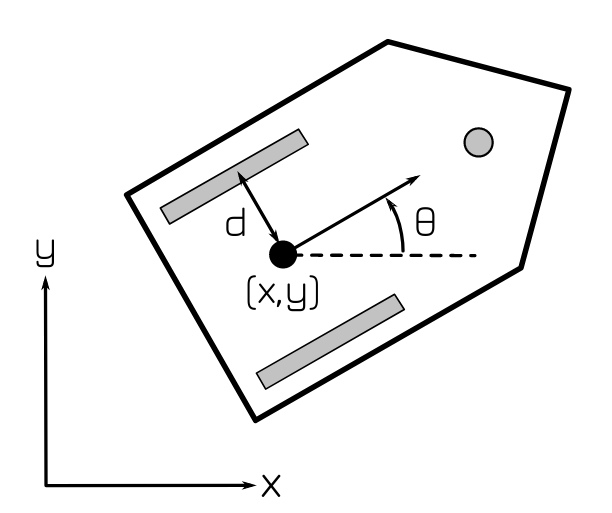
\includegraphics[width = 0.5\textwidth]{imgs/skid.png}
    \caption{Skid Drive Robot}
    \label{fig:skid-drive}
\end{figure}

In our kinematics, we assume that we can directly control the wheel velocities, $U_{l/r}$, where $U_l$ is our left wheel angular velocity and $U_r$ is our right wheel angular velocity. We have a variable $L$ which represents our wheelbase distance (between wheels) and $r$ which is our wheel radius. We use $L=0.4$ and $r=0.1$ in meters, estimating a large but still sidewalk-manageable delivery robot. For each kinematic step, we are looking at a set time increment, $\Delta t$.

\begin{equation}
    \dot{\theta} = \frac{r}{L}(U_r - U_)
\end{equation}
\begin{equation}
    \Delta \theta = \dot{\theta} \Delta t
\end{equation}
\begin{equation}
    \theta = \theta_0 + \Delta \theta
\end{equation}
\begin{equation}
    \dot{x} = \frac{r}{2}(U_r + U_l)\cos(\theta)
\end{equation}
\begin{equation}
    \dot{y} = \frac{r}{2}(U_r + U_l)\sin(\theta)
\end{equation}
\begin{equation}
    \Delta x = \dot{x} \Delta t
\end{equation}
\begin{equation}
    \Delta y = \dot{y} \Delta t
\end{equation}
\begin{equation}
    x = x_0 + \Delta x
\end{equation}
\begin{equation}
    y = y_0 + \Delta y
\end{equation}

\subsection*{Ackermann}

For our robot with Ackermann drive, we have two steerable wheels whose angle are mechanically linked and equivalent. Our rear wheels provide thrust, thus creating a different style of movement from our skid drive. We can no longer turn within our own radius, denoting a need for the path planner to perform K-turns and other maneuvers.

\begin{figure}[H]
    \centering
    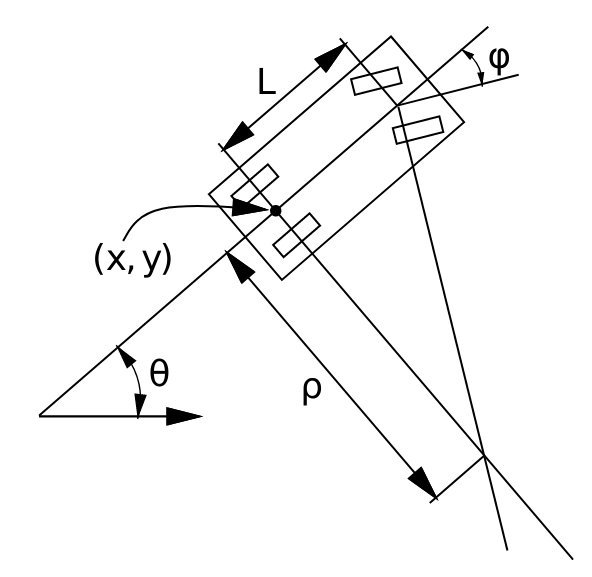
\includegraphics[width = 0.5\textwidth]{imgs/ackermann.png}
    \caption{Ackermann Drive Robot}
    \label{fig:ackermann-drive}
\end{figure}

The kinematics of our Ackermann drive robot can be expressed utilizng a controlled velocity $v$. Our steering is controllable as well, expressed as an agle $\psi$. For our robot, we chose a wheelbase $L=2.8$ meters. We allow a maximum $\lvert \psi \rvert = 60^\circ$.

\begin{equation}
    \dot{\theta} = \frac{v}{L} \tan(\psi)
\end{equation}
\begin{equation}
    \Delta \theta = \dot{\theta} \Delta t
\end{equation}
\begin{equation}
    \theta = \theta_0 + \Delta \theta
\end{equation}
\begin{equation}
    \dot{x} = v \cos(\theta)
\end{equation}
\begin{equation}
    \dot{y} = v \sin(\theta)
\end{equation}
\begin{equation}
    \Delta x = \dot{x} \Delta t
\end{equation}
\begin{equation}
    \Delta y = \dot{y} \Delta t
\end{equation}
\begin{equation}
    x = x_0 + \Delta x
\end{equation}
\begin{equation}
    y = y_0 + \Delta y
\end{equation}

\subsection*{Ackermann with a Trailer}

We expand our exploration of Ackermann drive robots by adding a hitched trailer, as if our robot was a large truck. The trailer has no control over its movement or velocity - it is pulled at an angle $\theta_1$ relative to the movement of the towing robot. For this assignment we only explored a singular trailer.

\begin{figure}[H]
    \centering
    
\includegraphics[width = 0.5\textwidth]{imgs/ackermann_trailer.png}
    \caption{Ackermann Drive Robot with Trailer}
    \label{fig:ackermann-drive-trailer}
\end{figure}

We assume a wheelbase $L=3$ meters and the distance of the trailer hitch to the center of rotation for the robot for a $d=5$ meters.

\begin{equation}
    \dot{\theta}_0 = \frac{v}{L} \tan(\psi)
\end{equation}
\begin{equation}
    \Delta \theta_0 = \dot{\theta}_0 \Delta t
\end{equation}
\begin{equation}
    \theta_0 = \theta_{0_0} + \Delta \theta_0
\end{equation}
\begin{equation}
    \dot{x} = v \cos(\theta_0)
\end{equation}
\begin{equation}
    \dot{y} = v \sin(\theta_0)
\end{equation}
\begin{equation}
    \Delta x = \dot{x} \Delta t
\end{equation}
\begin{equation}
    \Delta y = \dot{y} \Delta t
\end{equation}
\begin{equation}
    x = x_0 + \Delta x
\end{equation}
\begin{equation}
    y = y_0 + \Delta y
\end{equation}
\begin{equation}
    \dot{\theta}_1 = \frac{v}{d}\sin(\theta_0 - \theta_1)
\end{equation}
\begin{equation}
    \Delta \theta_1 = \dot{\theta}_1 \Delta t
\end{equation}
\begin{equation}
    \theta_1 = \theta_{1_0} + \Delta \theta_1
\end{equation}

The $(x,y)$ of the trailer is calculated from the resulting $\theta_1$ as the distance from the center of rotation for the trailer and truck is a set $d$ meters.

\section*{Planner Approach}

Here we present a flow chart for the path planner as built. We utilize an A* search algorithm. The act of expanding neighboring cells utilizes kinematic equations for each step to create an in-memory state lattic - this allows us to explore the continuous space as if it was a discrete space.

To store the state lattice and explore its nodes we implemented a priority queue. The cost of each node differs for each robot type, but typically is the euclidean distance between states from start to this point, and a penalty for $\theta$ changes (to encourage straight movement versus swerving when possible). For a heuristic, we heavily penalize euclidean distance ot the goal.

We are not exploring a discrete space, creating a need to identify an acceptable method of determining equality between nodes. To this end, we consider the node an equivalent state within a reasonable delta for $\Delta x$, $\Delta y$, and $\Delta \theta$. If the discovered state is within these bounds to an existing state, we would consider them equivalent.

Since we are taking discrete intervals when looking at $v$ velocity and $\psi$ steering angle, it is possible that we are near the goal but our chosen intervals can not generate a state transition that would be considered equivalent. To this end, we have introduced an extra step wherein we consider if the goal is reachable within the given $\Delta t$ time increment specified. We do this by considering distance between the goal and the current node, then back-calculating the required $U_r$, $U_l$, $v$, and $psi$, robot dependent, for a state transition to the desired spot. If the calculated potential inputs fall within the limits we specified for our robots, then the jump is possible and we can end our search here.

\begin{figure}[H]
    \centering
    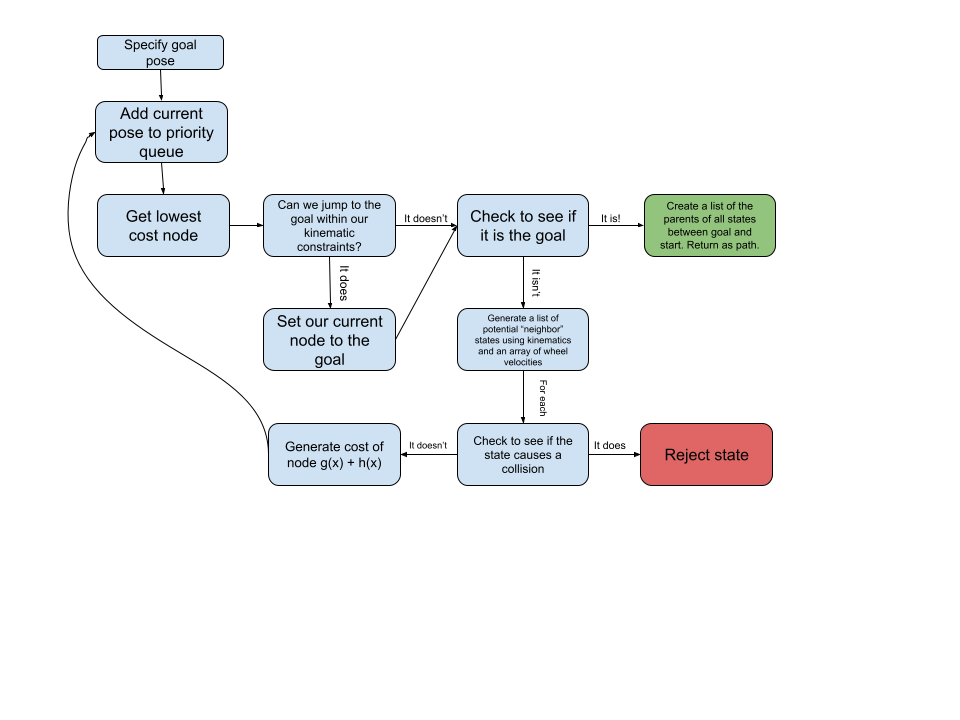
\includegraphics[width = 0.75\textwidth]{imgs/RBE550 Valet flow chart.png}
    \caption{Path planning flow chart}
    \label{fig:path-planning-flowchart}
\end{figure}

\section*{Results}

Here we provide examples of a path being generated to match a requested pose in an obstacle-laden environment. Each dot represents a considered state reached via the kinematic equations described above. The green line represents a path dictating which states ultimately led to the goal pose. We provide two examples for each vehicle.

\begin{figure}[H]
    \centering
    \begin{subfigure}{0.4\textwidth}
        \centering
        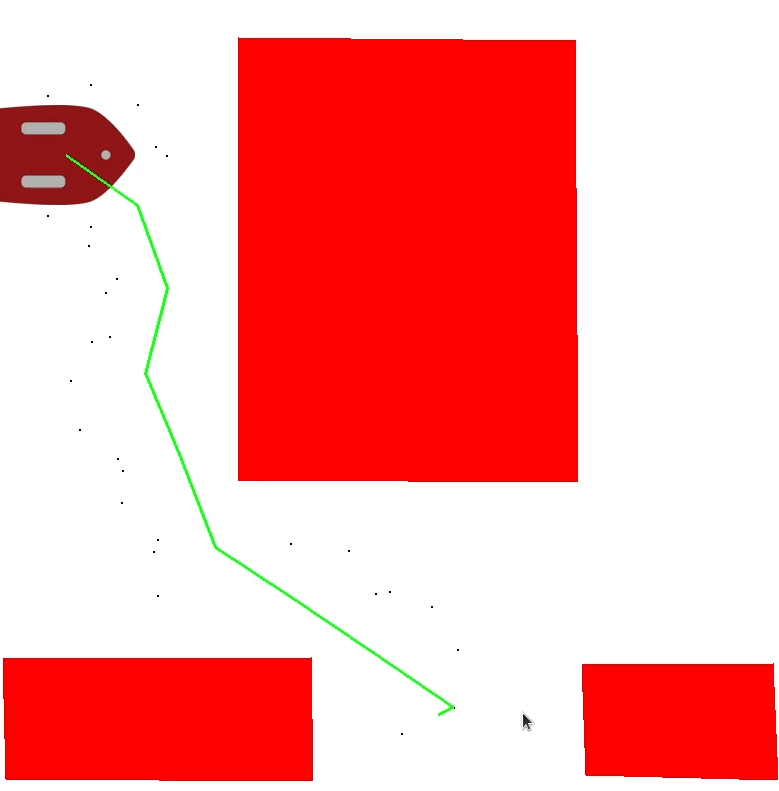
\includegraphics[width = \textwidth]{imgs/path_skid_1.png}
    \end{subfigure}
    \begin{subfigure}{0.4\textwidth}
        \centering
        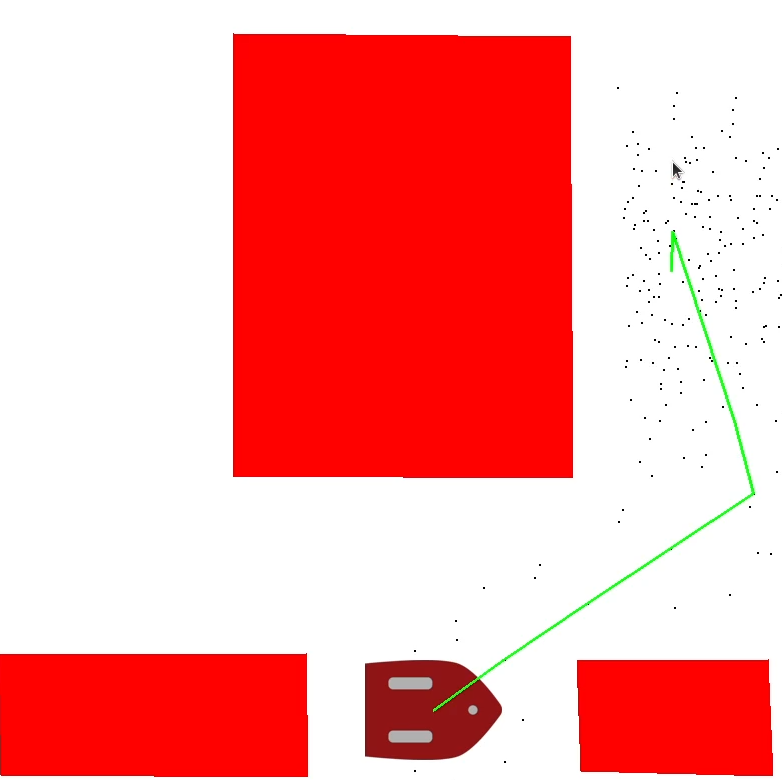
\includegraphics[width = \textwidth]{imgs/path_skid_2.png}
    \end{subfigure}
    \caption{Skid Drive Robot Path Planning}
    \label{fig:skid-drive-path}
\end{figure}

\begin{figure}[H]
    \centering
    \begin{subfigure}{0.4\textwidth}
        \centering
        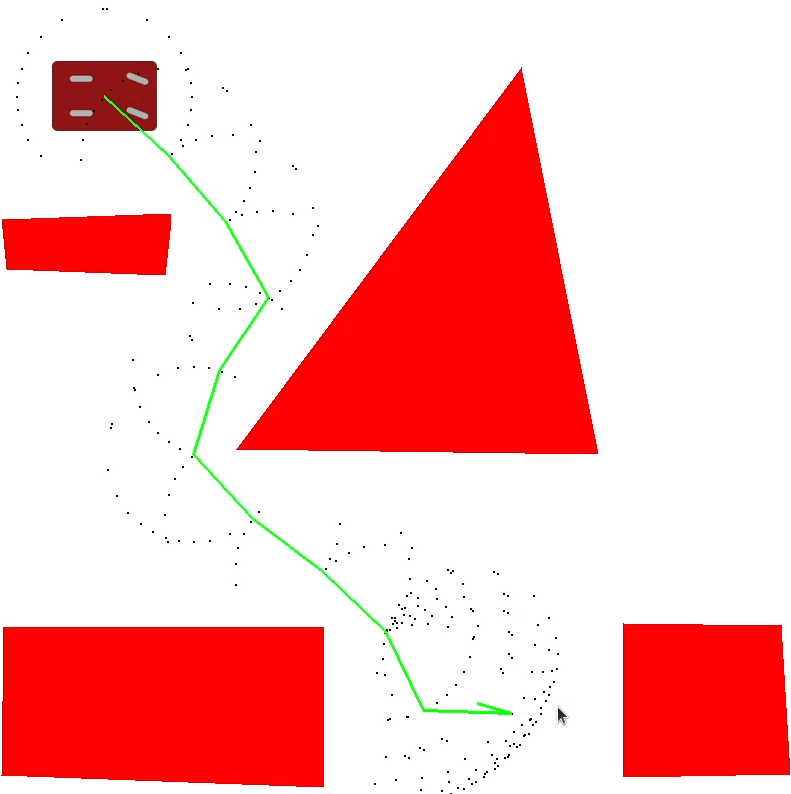
\includegraphics[width = \textwidth]{imgs/path_ackermann_1.png}
    \end{subfigure}
    \begin{subfigure}{0.4\textwidth}
        \centering
        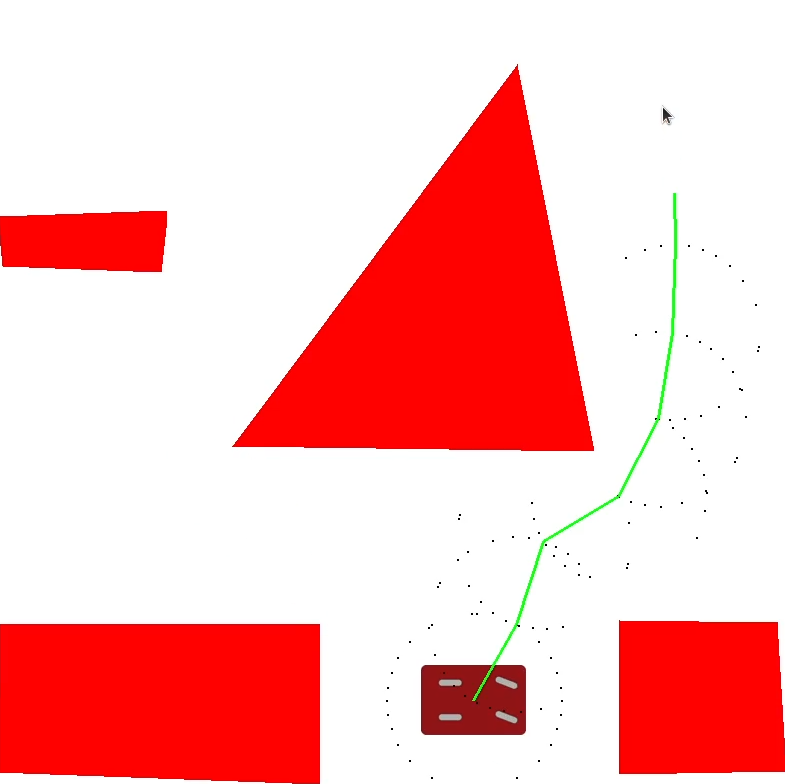
\includegraphics[width = \textwidth]{imgs/path_ackermann_2.png}
    \end{subfigure}
    \caption{Ackermann Robot Path Planning}
    \label{fig:ackermann-drive-path}
\end{figure}

\begin{figure}[H]
    \centering
    \begin{subfigure}{0.4\textwidth}
        \centering
        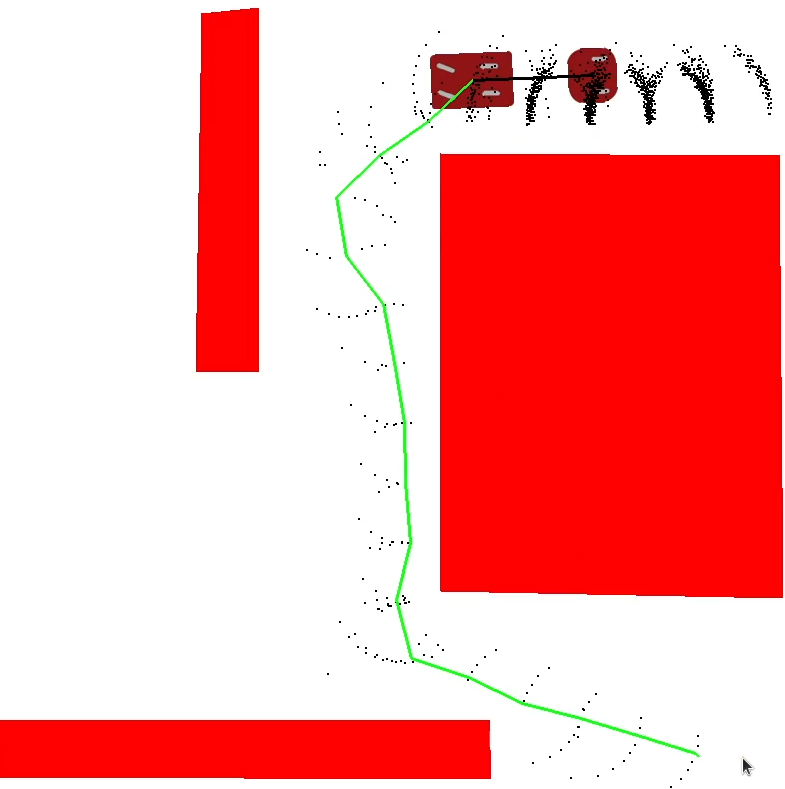
\includegraphics[width = \textwidth]{imgs/path_trailer_1.png}
    \end{subfigure}
    \begin{subfigure}{0.4\textwidth}
        \centering
        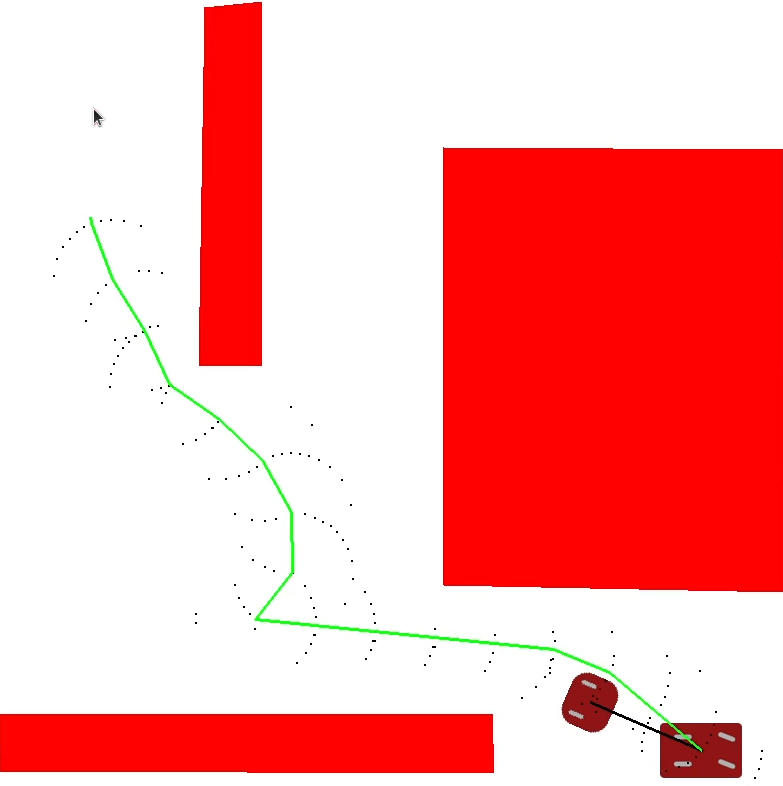
\includegraphics[width = \textwidth]{imgs/path_trailer_2.png}
    \end{subfigure}
    \caption{Ackermann Robot with Trailer Path Planning}
    \label{fig:ackermann-trailler-path}
\end{figure}

\section*{Conclusions}

In this assignment we created a path planning algorithm that worked in a continuous space utilizing the unique kinematic properties and constraints for each explored vehicle type.

We successfully managed to manuever around the continuous environment while avoiding collisions with obstacles.

During the completion of this project, several challenges were encountered. Our attempts to discretize the continuous space could improve, as we regularly see repeated exploration of previously explored areas; it is difficult to identify and confirm that you've considered a given area prior since we can not purely discretize a given space. This is due to our chosen method of determining if we've visited a space or not - storing nodes within a dict object. We utilized rounding of the state and overriding the default Python hashing functions to attempt to rectify this, but it still needs improvement to optimize performance.

We also witnessed the "tunneling" problem - since we move the vehicle with a given time increment, performing collision checks only at the start and finish poses for a given increment in the planner, we see chosen paths have small momentary collisions occasionally. Checking smaller intervals or performing collision checks for each intermediate step would be computationally expensive, but could be possible solutions.

We also see our simulation occasionally move oddly, identifiable as "sliding". This is due to our methodology of animating changes between poses. When animating our calculated pose, we utilize linear extrapolation of a given delta pose's $(x, y, \theta)$ instead of the actual curved trajectory that would have been performed. This was ignored as our simulation was acceptable enough for the time constraints.

It is this author's opinion that A* was, at times, not suitable for exploring the environment. There were times where a complicated environment would result in the algorithm exploring a given area too thoroughly, especially with our problems discretizing the continuous space. Algorithms that are more thorough in exploration, such as RRT*, could have performed better. We could have improved A* performance by experimenting with other node transition and heuristic costs as well.

Finally, our costs for each node ignored the presence and proximity to obstacles. Considering obstacle's proximity, such as using a gradient for the map where obstacles cause large peaks, would outperform our system for moving too close to obstacles, or would be more rapid about moving around obstacles.

\end{document}